%********************************************************************
% Appendix
%*******************************************************
% If problems with the headers: get headings in appendix etc. right
%\markboth{\spacedlowsmallcaps{Appendix}}{\spacedlowsmallcaps{Appendix}}
\chapter{Appendix}

\section{Appendix A: Datasets}\label{app:a}

There are a number of datasets used in the lab exercises and this appendix lists the following information about those datasets: 

\begin{enumerate}
  \item Type of data (Nominal, Ordinal, Interval, Ratio)
  \item Whether the data are normally distributed
  \item Skew
  \item Kurtosis
\end{enumerate}

\subsection{bdims}

This is a dataset of the body girth measurements and skeletal diameter measurements, as well as age, weight, height and gender, for $ 507 $ physically active individuals, $ 247 $ men and $ 260 $ women.

\begin{itemize}
  \item \textbf{age}. (Ratio : Normal : $ 1.131 $ : $ 0.96 $) The patient's age in years.  
  \item \textbf{ank.di}. (Ratio : Normal : $ 0.07 $ : $ -0.372 $) The patient's ankle diameter in centimeters, measured as sum of two ankles.
  \item \textbf{ank.gi}. (Ratio : Normal : $ 1.131 $ : $ 0.96 $) The patient's ankle minimum girth in centimeters, measured as average of right and left girths.  
  \item \textbf{bia.di}. (Ratio : Normal : $ 1.156 $ : $ -0.83 $) The patient's biacromial (shoulder width) in centimeters.
  \item \textbf{bic.gi}. (Ratio : Normal : $ 0.221 $ : $ -0.821 $) The patient's bicep girth in centimeters, measured when flexed as the average of right and left girths.
  \item \textbf{bii.di}. (Ratio : Normal : $ -0.417 $ : $ 1.09 $) The patient's biiliac (pelvic width) in centimeters.
  \item \textbf{bit.di}. (Ratio : Normal : $ -0.087 $ : $ 0.036 $) The patient's bitrochanteric (femur width) in centimeters.
  \item \textbf{cal.gi}. (Ratio : Normal : $ 0.278 $ : $ 0.301 $) The patient's calf maximum girth in centimeters, measured as average of right and left girths.  
  \item \textbf{che.de}. (Ratio : Normal : $ 0.495 $ : $ -0.128 $) The patient's chest depth in centimeters, measured between spine and sternum at nipple level, mid-expiration.
  \item \textbf{che.di}. (Ratio : Normal : $ 0.259 $ : $ -0.727 $) The patient's chest diameter in centimeters, measured at nipple level, mid-expiration.
  \item \textbf{che.gi}. (Ratio : Normal : $ 0.239 $ : $ -0.879 $) The patient's chest girth in centimeters, measured at nipple line in males and just above breast tissue in females, mid-expiration.
  \item \textbf{elb.di}. (Ratio : Normal : $ 0.053 $ : $ -0.731 $) The patient's elbow diameter in centimeters, measured as sum of two elbows.
  \item \textbf{for.gi}. (Ratio : Normal : $ 0.153 $ : $ -0.972 $) The patient's forearm girth in centimeters, measured when extended, palm up as the average of right and left girths.
  \item \textbf{hgt}. (Ratio : Normal : $ 0.152 $ : $ -0.45 $) The patient's height in centimeters.
  \item \textbf{hip.gi}. (Ratio : Normal : $ 0.498 $ : $ 0.774 $) The patient's hip girth in centimeters, measured at at level of bitrochanteric (femur width) diameter.
  \item \textbf{kne.di}. (Ratio : Normal : $ 0.341 $ : $ 0.081 $) The patient's knee diameter in centimeters, measured as sum of two knees.
  \item \textbf{kne.gi}. (Ratio : Normal : $ 0.469 $ : $ 1.019 $) The patient's knee diameter in centimeters, measured as sum of two knees.
  \item \textbf{nav.gi}. (Ratio : Normal : $ 0.45 $ : $ 0.14 $) The patient's navel (abdominal) girth in centimeters, measured at umbilicus and iliac crest using iliac crest as a landmark.
  \item \textbf{sex}. (Nominal : Not Normal : N/A : N/A) The patient's sex.
  \item \textbf{sho.gi}. (Ratio : Normal : $ 0.14 $ : $ -0.896 $) The patient's shoulder girth in centimeters, measured over deltoid muscles.
  \item \textbf{thi.gi}. (Ratio : Normal : $ 0.691 $ : $ 0.731 $) The patient's thigh girth in centimeters, measured below gluteal fold as the average of right and left girths.
  \item \textbf{wai.gi}. (Ratio : Normal : $ 0.541 $ : $ -0.218 $) The patient's waist girth in centimeters, measured at the narrowest part of torso below the rib cage as average of contracted and relaxed position.  
  \item \textbf{wgt}. (Ratio : Normal : $ 0.402 $ : $ -0.348 $) The patient's weight in kilograms.
  \item \textbf{wri.di}. (Ratio : Normal : $ 0.048 $ : $ -0.483 $) The patient's wrist diameter in centimeters, measured as sum of two wrists.
  \item \textbf{wri.gi}. (Ratio : Normal : $ 0.152 $ : $ -0.719 $) The patient's wrist minimum girth in centimeters, measured as average of right and left girths.  
\end{itemize}

\subsection{births}

This is a random sample of $ 1000 $ births in North Carolina in $ 2004 $.

\begin{itemize}
  \item \textbf{Fage}. (Ratio : Normal : $ 0.292 $ : $ -0.246 $) The father's age.
  \item \textbf{Fageord}. (Ordinal : Not Normal : N/A : N/A) Father's age groups. This is not in the original dataset and was added via recoding.
  \item \textbf{Gained}. (Ratio : Normal : $ 0.461 $ : $ 0.752 $) The mother's weight gain, in pounds.
  \item \textbf{Gainedord}. (Ordinal : Not Normal : N/A : N/A) Weight gained groups. This is not in the original dataset and was added via recoding.  
  \item \textbf{Gender}. (Nominal : Not Normal : N/A : N/A) The gender of the baby.
  \item \textbf{Habit}. (Nominal : Not Normal : N/A : N/A) Whether the mother was a smoker.
  \item \textbf{Lowbirthweight}. (Nominal : Not Normal : N/A : N/A) Whether the baby had a low birth weight.
  \item \textbf{Mage}. (Ratio : Normal : $ 0.263 $ : $ -0.636 $) The mother's age.
  \item \textbf{Mageord}. (Ordinal : Not Normal : N/A : N/A) Mother's age groups. This is not in the original dataset and was added via recoding.  
  \item \textbf{Marital}. (Nominal : Not Normal : N/A : N/A) Whether the mother was married.
  \item \textbf{Mature}. (Nominal : Not Normal : N/A : N/A) The mother's maturity status.
  \item \textbf{Premie}. (Nominal : Not Normal : N/A : N/A) Whether the baby was premature.
  \item \textbf{Visits}. (Interval : Normal : $ 0.263 $ : $ -0.636 $) The number of hospital visits made by the mother.
  \item \textbf{Weeks}. (Interval : Normal : $ -2.016 $ : $ 7.681 $) Length of pregnancy, in weeks. This data are normally distributed, but the skew and kurtosis are very poor so the data may be better treated as not normal.
  \item \textbf{Weight}. (Interval : Normal : $ -1.145 $ : $ 2.7 $) Birth weight of the baby, in pounds.
  \item \textbf{Whitemom}. (Nominal : Not Normal : N/A : N/A) Whether the mother was white.
\end{itemize}

\subsection{cars}

This is a random sample for $ 1993 $ model cars that were in both \textit{Consumer Reports} and \textit{PACE Buying Guide}. Only vehicles of type ``small,'' ``midsize,'' and ``large'' were included. The dataset has $ 54 $ rows and these data elements for each row:

\begin{itemize}
  \item \textbf{driveTrain}. (Nominal : Not Normal : N/A : N/A) Vehicle drive train with levels 4WD, front, and rear.
  \item \textbf{mpgCity}. (Ratio : Normal : $ 1.45 $ : $ 1.968 $) City mileage (miles per gallon).
  \item \textbf{passengers}. (Ordinal : Not Normal : N/A : N/A) The vehicle passenger capacity. 
  \item \textbf{price}. (Ratio : Normal : $ 1.327 $ : $ 1.897 $) Vehicle price in U.S. dollars.
  \item \textbf{type}. (Ordinal : Not Normal : N/A : N/A) The vehicle type with levels large, midsize, and small.
  \item \textbf{weight}. (Ratio : Normal : $ -0.233 $ : $ -1.168 $) Vehicle weight in pounds. The skew and kurtosis for this data are good, but the histogram is rather flat. This may be better considered a not normal distribution.
\end{itemize}

\subsection{doorsurvey}

\textit{This is simulated data.} Students recorded observations about the customers entering a store between $ 9 $ AM and $ 11 $ AM for a one week period.

\begin{itemize}
  \item \textbf{agecat}. (Ordinal : Not Normal : N/A : N/A) An estimate of the age category for the customer where $ 1 $ is less than $ 30 $ years old, $ 2 $ is between $ 30 $ and $ 50 $ years old, and $ 3 $ is more than $ 50 $ years old. If a group entered then the age of the first adult in the group was estimated.
  \item \textbf{day}. (Ordinal : Not Normal : N/A : N/A) The date the customers were observed.
  \item \textbf{grpnum}. (Ordinal : Not Normal : N/A : N/A) The number of people in the group.
  \item \textbf{gender}. (Nominal : Not Normal : N/A : N/A) The sex of the customer: \textit{m} or \textit{f}. If a group entered then the sex of the first adult in the group was recorded.
\end{itemize}

\subsection{email}

This dataset contains $ 3154 $ observations from the email received by one person over a period of several months in $ 2012 $.

\begin{itemize}
  \item \textbf{attach}. (Ratio : Not Normal : $ 16.278 $ : $ 502.528 $) The number of attached files. 
  \item \textbf{cc}. (Ratio : Not Normal : $ 13.51 $ : $ 225.074 $) How many people were CCed on the message.
  \item \textbf{dollar}. (Ratio : Not Normal : $ 4.456 $ : $ 22.826 $) The number of times a dollar sign or the word ``dollar'' appeared in the email.
  \item \textbf{exclaim\_mess}. (Ratio : Not Normal : $ 4.107 $ : $ 23.946 $) The number of exclamation points in the email message.
  \item \textbf{exclaim\_subj}. (Nominal : Not Normal : N/A : N/A) \textit{No} if the email subject did not have an exclamation point, otherwise \textit{yes}.
  \item \textbf{format}. (Nominal : Not Normal : N/A : N/A) \textit{Text} if the message was sent in text format and \textit{html} if it used HTML format.
  \item \textbf{image}. (Ratio : Not Normal : $ 9.621 $ : $ 121.313 $) The number of images attached.
  \item \textbf{inherit}. (Ratio : Not Normal : $ 18.188 $ : $ 478.488 $) The number of times ``inherit'' (or an extension, such as ``inheritance'') appeared in the email.
  \item \textbf{line\_breaks}. (Ratio : Normal : $ 0.974 $ : $ 0.046 $) The number of line breaks in the email (does not count text wrapping).
  \item \textbf{num\_char}. (Ratio : Normal : $ 0.944 $ : $ -0.017 $) The number of characters in the email, in thousands.
  \item \textbf{number} (Ordinal : Not Normal : N/A : N/A) \textit{None} if the message included no numbers, \textit{small} if it included only numbers less than one million, or \textit{large} if it included one or more big numbers.
  \item \textbf{password}. (Ratio : Not Normal : $ 16.173 $ : $ 333.185 $) The number of times ``password'' appeared in the email.
  \item \textbf{re\_subj}. (Nominal : Not Normal : N/A : N/A) \textit{No} if the subject did not include any of these: ``Re:'', ``RE:'', ``re:'', or ``rE:'', otherwise \textit{yes}.
  \item \textbf{sent\_email}. (Nominal : Not Normal : N/A : N/A) \textit{No} if no email was sent to the sender in the last $ 30 $ days, otherwise \textit{yes}.
  \item \textbf{spam}. (Nominal : Not Normal : N/A : N/A) \textit{Yes} if the message is spam, otherwise \textit{no}.
  \item \textbf{spamnum}. (Ordinal : Not Normal : N/A : N/A)  Numeric representation of the ``spam'' data item. This is not in the original dataset and was added via recoding.
  \item \textbf{to\_multiple}. (Nominal : Not Normal : N/A : N/A) \textit{No} for mail that was sent to only one person, otherwise \textit{yes}.
  \item \textbf{urgent\_subj}. (Nominal : Not Normal : N/A : N/A) \textit{Yes} if the subject included the word ``urgent,'' otherwise \textit{no}.
  \item \textbf{viagra}. (Ratio : Not Normal : $ 56.134 $ : $ 3149.0 $) The number of times ``viagra'' appeared in the email.
  \item \textbf{winner}. (Nominal : Not Normal : N/A : N/A) \textit{Yes} if the word ``winner'' appeared in the email, otherwise \textit{no}.
\end{itemize}

\subsection{gifted}

An investigator is interested in understanding the relationship, if any, between the analytical skills of young gifted children and the variables listed below. The analytical skills are evaluated using a standard testing procedure and the score on that test is included in the dataset. Data were collected from schools in a large city on a set of $ 36 $ children who were identified as gifted children soon after they reached the age of four.

\begin{itemize}
  \item \textbf{Cartoons}. (Ratio : Normal : $ 0.053 $ : $ -0.551 $) Average number of hours per week the child watched cartoons on TV during the past three months.
  \item \textbf{Count}. (Interval : Normal : $ -0.197 $ : $ -0.653 $) Age in months when the child first counted to ten successfully.
  \item \textbf{Edutv}. (Ratio : Normal : $ -0.053 $ : $ -0.375 $) Average number of hours per week the child watched an educational program on TV during the past three months.
  \item \textbf{Fatheriq}. (Interval : Normal : $ 1.091 $ : $ 1.459 $) Father's IQ.
  \item \textbf{Motheriq}. (Interval : Normal : $ 0.247 $ : $ 0.035 $) Mother's IQ.
  \item \textbf{Read}. (Ratio : Normal : $ -0.576 $ : $ -0.449 $) Average number of hours per week the child's mother or father reads to the child.
  \item \textbf{Score}. (Ratio : Normal : $ -0.016 $ : $ -0.528 $) The score in test of analytical skills.
  \item \textbf{Speak}. (Interval : Normal : $ -0.627 $ : $ -0.153 $) Age in months when the child first said ``mummy'' or ``daddy.''
\end{itemize}

\subsection{maincafe}

\textit{This is simulated data.} Customers of the Main Street Caf\'{e} completed surveys over a one week period. Note: this dataset is occasionally re-created so the values for skew and kurtosis are only estimates.

\begin{itemize}
  \item \textbf{age}. (Ratio : Normal : $ \approx 0.2 $ : $ \approx -0.6 $) The age in years of the person completing the survey.
  \item \textbf{bill}. (Interval : Normal : $ \approx 1.0 $ : $ \approx 0.5 $) The bill for the meal.
  \item \textbf{day}. (Nominal : Not Normal : N/A : N/A) The day of the week the person visited the cafe. The levels are written names of days, like ``Sunday'' and ``Monday.''
  \item \textbf{food}. (Ordinal : Not Normal : N/A : N/A) A rating for the food, from one to five ``stars.''
  \item \textbf{length}. (Interval : Normal : $ \approx -0.5 $ : $ \approx -0.2 $) The length of the visit in minutes.
  \item \textbf{meal}. (Nominal : Not Normal : N/A : N/A) The meal eaten stored as Breakfast, Lunch, Dinner, and Other.
  \item \textbf{miles}. (Interval : Not Normal : $ \approx 8.2 $ : $ \approx 71.0 $) The number of miles from the visitor's home and the cafe.
  \item \textbf{pref}. (Nominal : Not Normal : N/A : N/A) A binary item for the preference in tables of the diner. The levels are ``table'' and ``booth.''
  \item \textbf{ptysize}. (Interval : Normal : $ \approx 0.7 $ : $ \approx 0.1 $) The size of the dining party.
  \item \textbf{recmd}. (Nominal : Not Normal : N/A : N/A) A binary item for whether the customer would recommend the caf\'{e} to other people, stored as ``no'' and ``yes.''   
  \item \textbf{sex}. (Nominal : Not Normal : N/A : N/A) The gender of the person completing the survey. The levels are: male, female, and other. 
  \item \textbf{svc}.  (Ordinal : Not Normal : N/A : N/A) A rating for the service, from one to five ``stars.''
  \item \textbf{tip}. (Ratio : Normal : $ \approx 1.4 $ : $ \approx 1.2 $) The amount of tip left.
\end{itemize}

\subsection{rivers}

The Rivers dataset is a list of the lengths of the longest $ 141 $ rivers in the United States. These data are not normally distributed.

\begin{quote}
  $ 135 $, $ 202 $, $ 210 $, $ 210 $, $ 215 $, $ 217 $, $ 230 $, $ 230 $, $ 233 $, $ 237 $, $ 246 $, $ 250 $, $ 250 $, $ 250 $, $ 255 $, $ 259 $, $ 260 $, $ 260 $, $ 265 $, $ 268 $, $ 270 $, $ 276 $, $ 280 $, $ 280 $, $ 280 $, $ 281 $, $ 286 $, $ 290 $, $ 291 $, $ 300 $, $ 300 $, $ 300 $, $ 301 $, $ 306 $, $ 310 $, $ 310 $, $ 314 $, $ 315 $, $ 320 $, $ 325 $, $ 327 $, $ 329 $, $ 330 $, $ 332 $, $ 336 $, $ 338 $, $ 340 $, $ 350 $, $ 350 $, $ 350 $, $ 350 $, $ 352 $, $ 360 $, $ 360 $, $ 360 $, $ 360 $, $ 375 $, $ 377 $, $ 380 $, $ 380 $, $ 383 $, $ 390 $, $ 390 $, $ 392 $, $ 407 $, $ 410 $, $ 411 $, $ 420 $, $ 420 $, $ 424 $, $ 425 $, $ 430 $, $ 431 $, $ 435 $, $ 444 $, $ 445 $, $ 450 $, $ 460 $, $ 460 $, $ 465 $, $ 470 $, $ 490 $, $ 500 $, $ 500 $, $ 505 $, $ 524 $, $ 525 $, $ 525 $, $ 529 $, $ 538 $, $ 540 $, $ 545 $, $ 560 $, $ 570 $, $ 600 $, $ 600 $, $ 600 $, $ 605 $, $ 610 $, $ 618 $, $ 620 $, $ 625 $, $ 630 $, $ 652 $, $ 671 $, $ 680 $, $ 696 $, $ 710 $, $ 720 $, $ 720 $, $ 730 $, $ 735 $, $ 735 $, $ 760 $, $ 780 $, $ 800 $, $ 840 $, $ 850 $, $ 870 $, $ 890 $, $ 900 $, $ 900 $, $ 906 $, $ 981 $, $ 1000 $, $ 1038 $, $ 1054 $, $ 1100 $, $ 1171 $, $ 1205 $, $ 1243 $, $ 1270 $, $ 1306 $, $ 1450 $, $ 1459 $, $ 1770 $, $ 1885 $, $ 2315 $, $ 2348 $, $ 2533 $
\end{quote}

\subsection{tutoring}

\textit{This is simulated data.} A professor designed an experiment where she first administered a pretest to all students. She then required all students to work with an online tutoring service every week. At the end of four weeks she administered a post-test and labeled the scores on that test as ``Test01.'' She then required students to attend weekly face-to-face tutoring sessions. After four weeks she administered a different, but similar, post-test and labeled the scores on that test as ``Test02.'' After each of the three tests she asked the students what grade they expected to earn. This dataset includes the test scores and grade predictions for each of the students.
 
\begin{itemize}
  \item \textbf{ExpGra01}. (Ordinal : Not Normal : N/A : N/A) This is the expected grade the student reported after Test01. The levels are A=$ 4 $, B=$ 3 $, C=$ 2 $, and D=$ 1 $.
  \item \textbf{ExpGra02}. (Ordinal : Not Normal : N/A : N/A) This is the expected grade the student reported after Test02. The levels are A=$ 4 $, B=$ 3 $, C=$ 2 $, and D=$ 1 $.
  \item \textbf{ExpGraPre}. (Ordinal : Not Normal : N/A : N/A) This is the expected grade the student reported during the pretest. The levels are A=$ 4 $, B=$ 3 $, C=$ 2 $, and D=$ 1 $.
  \item \textbf{Pretest}. (Ratio : Normal : $ 0.199 $ : $ -0.591 $) This is the student's pretest score.
  \item \textbf{StuID}. (Interval : Not Normal : N/A : N/A) This is just a one-up number assigned to identify each student in the study.
  \item \textbf{Test01}. (Ratio : Normal : $ 0.063 $ : $ -0.205 $) This is the score for students on the first post-test.
  \item \textbf{Test02}. (Ratio : Normal : $ -0.05 $ : $ -0.109 $) This is the score for students on the second post-test.
\end{itemize}

\section{Appendix B: Recoding Variables} \label{app:b}

\subsection{Background}

For efficiency, data are often stored in a database in a format that does not lend itself to easy analysis. For example, nominative values, like ``no'' and ``yes'' are frequently stored as $ 0 $ and $ 1 $. While that is efficient for storage it makes using a table or chart more difficult because the various data elements will be presented as something like $ 0 $ instead of ``no'' and it is incumbent upon the researcher to remember what the various codes mean; however, values in a dataset can be recoded to make them easier to use. As examples, ``$ 0 / 1 $'' values can be recoded to ``no/yes'' or a variable containing ages can be recoded so the ages are grouped, like ages $ 20 - 29 $ can be recoded to $ 2 $. 

\subsection{Recoding Variables With \texttt{SOFA}}

In \texttt{SOFA}, a data field is recoded into a new field so the dataset ends up with two fields that contain the same data but in different formats. As an example, imagine that a researcher is using the ``spam'' field of the \textit{email} dataset and desires to use $ 0 $ instead of ``no'' and $ 1 $ instead of ``yes,'' then that field would need to be recoded.

\begin{enumerate}
  \item {Start \texttt{SOFA} and select ``Enter/Edit Data.''}
  \item Data Tables: email
  \item Click ``Design''
  \item Click the ``Recode'' button on the Data Table screen
  \item Fill in the ``Recode'' screen as illustrated below. (Note: since each row is saved as it is entered, the cursor must be moved into Row $ 3 $, as illustrated, in order to save the changes made on Row $ 2 $).
  
  \begin{figure}[H]
    \begin{center}
      \fbox{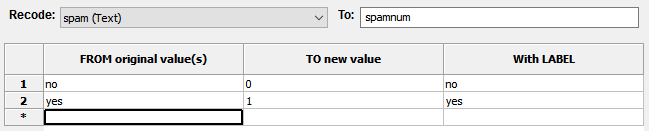
\includegraphics[width=\linewidth]{gfx/apb005}}
      \caption{Recoding Spam Field}
    \end{center}
  \end{figure}
  
  \item Click ``Recode''
  \item The following message will be displayed
  
  \begin{figure}[H]
    \begin{center}
      \fbox{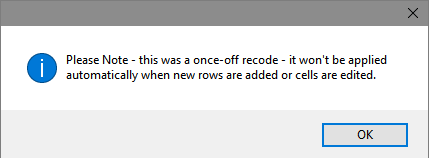
\includegraphics[]{gfx/apb010}}
      \caption{Recode Warning on Save}
    \end{center}
  \end{figure}
  
  \item Click OK to dismiss the warning, click OK to complete the recode, and then click ``Update'' to file the results of the recode process.

\end{enumerate}

When this process is completed the \textit{email} dataset will contain a new field named ``spamnum'' that contains a $ 0 $ where ``spam'' is equal to ``no'' and a $ 1 $ where ``spam'' is ``yes.''

\section{Appendix C: SOFA Exports} \label{app:c}

\texttt{SOFA} creates several different types of exports and each are easy to generate and use. Export specifications are set in the area across the center of the various pop-up windows (Report Tables, Charts, and Statistics) and generating reports is the same for all of the windows.

\subsection{Styles}

\texttt{SOFA} comes with seven built-in styles that can be selected from the box on the bottom-right of the window:

\begin{figure}[H]
  \begin{center}
    \fbox{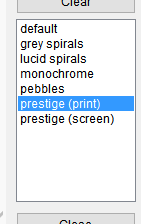
\includegraphics[]{gfx/apc005}}
    \caption{SOFA Styles}
  \end{center}
\end{figure}

As each style is selected the display in the lower-left corner of the window is immediately updated to reflect the selected style.

\subsection{Exporting a File}

The output in the lower-left corner of the window can be exported in a file that can be opened by a program like Excel. In the Export drop-down box at the right-center of the window select ``Current Output'' and then click the ``Export'' button.

\begin{figure}[H]
  \begin{center}
    \fbox{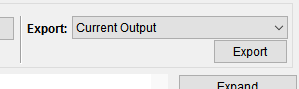
\includegraphics[]{gfx/apc010}}
    \caption{Selecting Export Type}
  \end{center}
\end{figure}

Select the specific type of output desired in the pop-up window.

\begin{figure}[H]
  \begin{center}
    \fbox{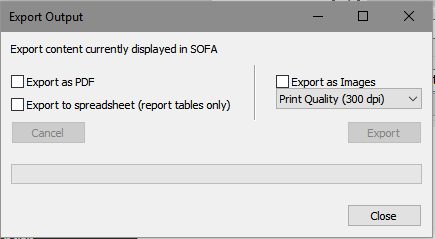
\includegraphics[]{gfx/apc015}}
    \caption{Specifying Desired Export}
  \end{center}
\end{figure}

\begin{itemize}
  \item Export as PDF. This option will generate a PDF file containing the current output. Note that a number of different outputs can be combined into a single PDF file by using the ``Report'' feature, described below.
  \item Export to spreadsheet (report tables only). This generates an Excel spreadsheet without any formatting. This is an excellent option if the data produced by \texttt{SOFA} needs further manipulation.
  \item Export as Images. \texttt{SOFA} will export the output as .PNG images that can be used in other programs or emailed. The quality of the image can be selected using the drop-down box. (NOTE: for most work the ``Print Quality (300 dpi)'' setting is adequate.)
\end{itemize}

Click the ``Export'' button to generate the desired export file.


\subsection{Copy/Paste Output}

In the dropdown ``Export'' box, select ``Copy current output ready to paste'' to copy the output displayed in the lower left corner of the window so it can be pasted directly into Word or some other program.

\subsection{Reports}

\texttt{SOFA} can combine the outputs for several operations into a single PDF report or series of .PNG files. This is a two-step process, first the various outputs are saved into a report and, second, the final report is exported.

To save the outputs into a single report, start by specifying the location and name for the report. By default, \texttt{SOFA} saves reports in the \textit{sofastats/reports} folder and that is appropriate since \texttt{SOFA} can generate a number of files when producing a report. To specify the name for a new report, click the ``Browse'' button and enter the report's name (it is the file name). \texttt{SOFA} saves reports in .HTM format but a different format can be specified when the report is later exported.

Then, as outputs are produced, click the ``Also add to report'' button to add the current output, displayed in the lower-left corner of the window, to the report. Note: every time the ``Also add to report'' button is clicked the current output is added to the report so avoid clicking that button multiple times unless multiple copies of the current output are desired.

To export the report, select ``Entire Report'' in the export drop-down box. Select the format for the report (PDF, images, or Excel Spreadsheet) and click ``Export.'' 

Note: SOFA exports PDF files such that each saved output screen is on a different PDF page, which makes the PDF file rather long with a lot of blank space between pages. As an alternative, it may be possible to click the ``View Report'' button to open the report in a browser and then use the browser's print feature.



